\documentclass{beamer}
\usepackage{./common_slides}
\usepackage[absolute,overlay]{textpos}
\usepackage{graphicx}


\title{ Reimplementing End-to-End Generative Dialogue }

\author{Michael Farrell, Colton Gyulay, Kevin Yang}
\begin{document}

\begin{frame}
  \titlepage
\end{frame}

\iffalse
\begin{frame}{Background (Literature Summary)}
\begin{itemize}
\item End to End Dialogue Systems
\begin{itemize}
\item  Implementation of encoder decoder system for conversations
\item Movie Triples Dataset
\item Describe Movie Triples Dataset setup
\item Around 160,000 training examples, 20,000 validation examples
\item Describe models and metrics
\end{itemize}
\item Include table of models and metrics
\end{itemize}
\end{frame}
\fi

\begin{frame}[fragile]{Objectives}

\begin{itemize}
\item Main focus of our project is to re-implement and explore extensions for the dialogue system described in Serban et al's (2016) paper: \textit{Building End-to-End Dialogue Systems Using Generative Hierarchical Neural Network Models}. 
\item Use the Movie Triples dataset. Dataset with around 200,000 utterance triples $(U_1, U_2, U_3)$. Goal is to predict $U_3$ given $U_1$ and $U_2$. \\
 \begin{verbatim} 
 U1: you lied to me so many times -- 
 U2: reggie -- trust me once more -- please . 
 U3: can i really believe you this time , <person> ? 
 \end{verbatim}
 \end{itemize}
\end{frame}

\begin{frame}{Objectives}
\begin{itemize}

\item For generating dialogue, authors of the paper use perplexity and error-rate.
\item They used a variety of different models for their encoder and decoder. Some of their results are shown below.\\
\begin{center}
\begin{figure}
\hspace*{-1cm}
 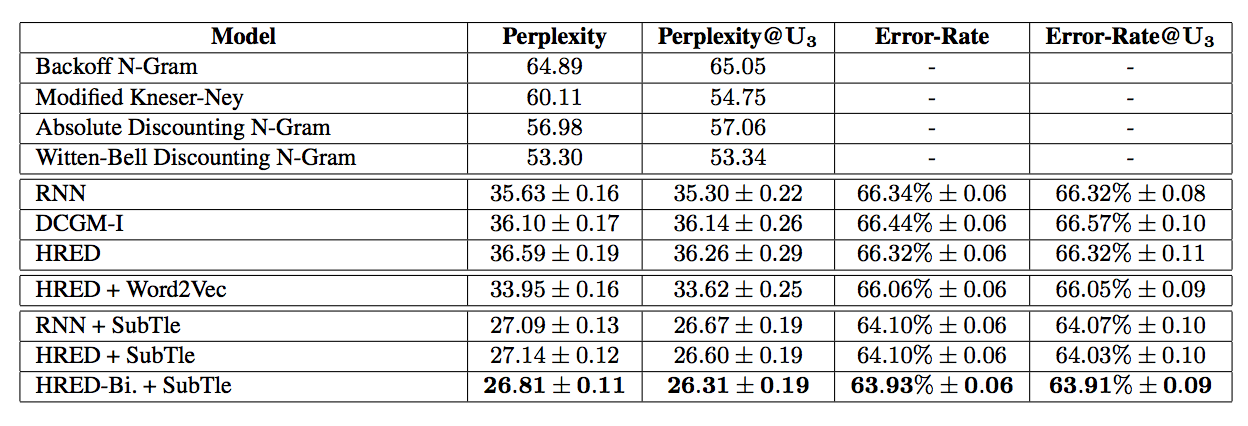
\includegraphics[scale = .4]{perp_table.png}
\end{figure}
\end{center}
\item The model that performs the best is the hierarchical encoder decoder (HRED) model.
\end{itemize}
\end{frame}

\begin{frame}{Hierarchical Encoder Decoder Model}
\begin{center}
$$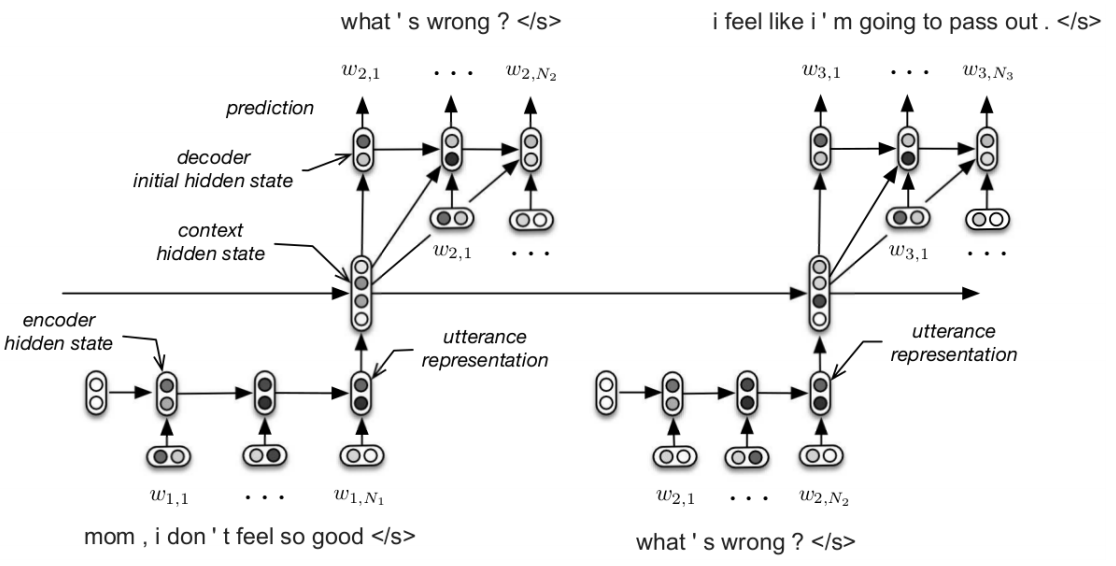
\includegraphics[scale = .6]{hred.png}$$
\end{center}
\end{frame}

\begin{frame}{Results}
\begin{itemize}
\item We reached out to Iulian Serban to get the Movie Triples dataset. Using the Element rnn library, we trained encoder and decoders with RNN, GRU, and LSTM layers. To generate predictions, we implemented and ran beam search. We also ran Yoon Kim's seq2seq-attn model \footnote{https://github.com/harvardnlp/seq2seq-attn/}.

\item Our best model had 2 stacked layers of LSTMs for both the encoder and the decoder with word2vec embeddings. Our validation perplexity reached a low of 38.2 after 10 epochs. This is comparable to results from Serban et al.'s models without bootstrapping from the SubTle dataset.

\end{itemize}
\end{frame}

\begin{frame}[fragile]{Results: Example Inputs and Outputs}
\begin{itemize}
\item Our results did suffer from similar issues that Serban et al. had though, where utterances were short and ambiguous. Generally, lower validation perplexity did not necessarily mean better results.\\


\begin{verbatim}
U1 : when do these boys of yours go on the road ?
U2: coupla weeks . for eight weeks .
Predicted U3:   1) that ' s right .
                2) that ' s not the point .
                3) that ' s not what i meant .
                4) that ' s what i ' m talking about .
                5) that ' s what i ' m saying .
    
Actual U3: that ' s a nice tour . all booked ?
\end{verbatim}

\end{itemize}
\end{frame}

\begin{frame}[fragile]{Results: Example Inputs and Outputs}
\begin{itemize}

\begin{verbatim}
U1 : me too . we ' d love to have you . 
U2: you know, this is the best pie i ' ve ever had .
Predicted U3:   1) <person> .
                2) i don't know
                3) i'm sorry
                4) that's good
                5) i don't know what
    
Actual U3: oh? 
\end{verbatim}
\end{itemize}

\end{frame}


\begin{frame}{Results: Speeding Up Training}

\begin{itemize}
\item The major bottleneck for training these models was time. Training a single epoch on a Macbook Pro with an NVIDIA GeForce 750M took around 3 hours per epoch.
\item In order to expedite this process, we applied the lua-parallel \footnote{https://github.com/clementfarabet/lua---parallel} module to the problem. This produces a 4x speedup with CPU. Currently, we're trying to extend this module across multiple Google Cloud Compute instances to further increase the speed of training.
\end{itemize}
\end{frame}


\begin{frame}{Further Extensions}
\begin{itemize}
\item We would like to experiment with the HRED model and see if it achives similar results to Serban et al's results. 
\item After implementing a distributed way to train models, we would like to do some parameter tuning and work with the SuBtle dataset.
\item We would like to experiment with adding more context into the model. Currently, we're only using two utterances as context. 
\item Finally, we would like to try to generate more interesting conversation output.
\end{itemize}
\end{frame}

\end{document}
